\documentclass[tikz,border=4pt]{standalone}
\usepackage[T1]{fontenc}
\usepackage{lmodern}
\renewcommand{\familydefault}{\sfdefault}
\usetikzlibrary{shapes.geometric,positioning,arrows.meta,calc}
\tikzset{
  node distance=6mm,
  every node/.style={font=\footnotesize,align=center,execute at begin node={\hyphenpenalty=10000\relax}},
  base/.style={draw=gray!60,fill=gray!12,minimum height=7mm,inner sep=2pt},
  term/.style={base,rounded corners=3.5mm,text width=30mm},
  proc/.style={base,text width=32mm},
  err/.style={base,text width=30mm,fill=gray!22},
  io/.style={base,trapezium,trapezium left angle=72,trapezium right angle=108,trapezium stretches=true,text width=28mm},
  dec/.style={base,diamond,aspect=2.4,text width=27mm,inner sep=0pt},
  go/.style={-{Stealth[length=2mm]},draw=gray!55!black},
  lab/.style={font=\scriptsize,fill=white,inner sep=1pt},
}

\begin{document}
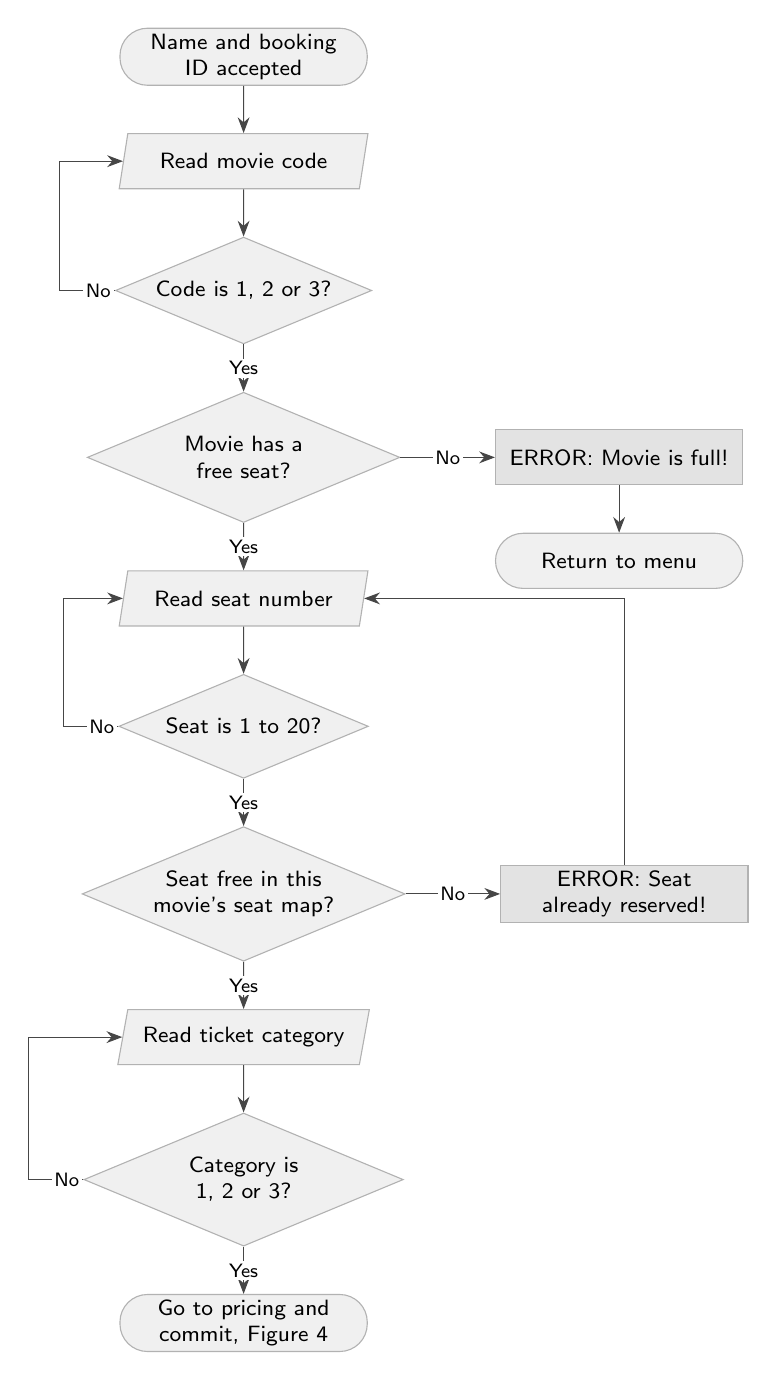
\begin{tikzpicture}
\node[term] (s) {Name and booking ID accepted};
\node[io,below=of s] (m) {Read movie code};
\node[dec,below=of m] (d1) {Code is 1, 2 or 3?};
\node[dec,below=of d1] (f) {Movie has a free seat?};
\node[err,right=12mm of f] (e0) {ERROR: Movie is full!};
\node[term,below=of e0] (r) {Return to menu};
\node[io,below=of f] (t) {Read seat number};
\node[dec,below=of t] (d2) {Seat is 1 to 20?};
\node[dec,below=of d2] (d3) {Seat free in this movie's seat map?};
\node[err,right=12mm of d3] (e1) {ERROR: Seat already reserved!};
\node[io,below=of d3] (c) {Read ticket category};
\node[dec,below=of c] (d4) {Category is 1, 2 or 3?};
\node[term,below=of d4] (g) {Go to pricing and commit, Figure 4};
\draw[go] (s)--(m);\draw[go] (m)--(d1);
\draw[go] (d1)--node[lab]{Yes}(f);
\draw[go] (d1.west)--node[lab,pos=.3]{No}++(-7mm,0)|-(m.west);
\draw[go] (f)--node[lab]{Yes}(t);
\draw[go] (f)--node[lab]{No}(e0);
\draw[go] (e0)--(r);
\draw[go] (t)--(d2);
\draw[go] (d2)--node[lab]{Yes}(d3);
\draw[go] (d2.west)--node[lab,pos=.3]{No}++(-7mm,0)|-(t.west);
\draw[go] (d3)--node[lab]{Yes}(c);
\draw[go] (d3)--node[lab]{No}(e1);
\draw[go] (e1.north)|-(t.east);
\draw[go] (c)--(d4);
\draw[go] (d4)--node[lab]{Yes}(g);
\draw[go] (d4.west)--node[lab,pos=.3]{No}++(-7mm,0)|-(c.west);
\end{tikzpicture}
\end{document}
